\documentclass[12pt]{article}
\usepackage{amsmath}
\usepackage{multirow}
\usepackage{enumerate}
\usepackage{graphicx}
\usepackage{changepage}
\usepackage[all]{xy}
\usepackage{tikz}
\usetikzlibrary{shapes}


\setlength{\voffset}{-3cm}
%\setlength{\hoffset}{-2cm}
%\setlength{\parindent}{0cm}
\setlength{\textheight}{26cm}
%\setlength{\textwidth}{14cm}


\begin{document}


\begin{center}

\includegraphics[width=0.6\textwidth]{ul_logo}
\quad\\[1cm]
{\bf\large FACULTY OF SCIENCE AND ENGINEERING\\[0.5cm]}
{\bf\small DEPARTMENT OF MATHEMATICS AND STATISTICS\\[0.8cm]}
{\large END OF SEMESTER ASSESSMENT PAPER\\[2cm]}
\begin{adjustwidth}{-1cm}{0cm}
\begin{tabular}{l@{\qquad}l}
MODULE CODE: MA4413&SEMESTER: Autumn 2015\\[1cm]
MODULE TITLE: Statistics for Computing& DURATION OF EXAM: 2.5 hours\\[1cm]
LECTURER: Dr.~Kevin Burke& GRADING SCHEME: 100 marks \\
& \hspace{3cm} (60\% of module)\\[2cm]
%EXTERNAL EXAMINER:&\\
%Prof. Brendan Murphy&\\[1cm]
\end{tabular}
\end{adjustwidth}
{\bf INSTRUCTIONS TO CANDIDATE}
\end{center}
\begin{small}
\begin{itemize}\itemsep0.3cm
\item {\bf Attempt four} of the six questions (each one carries 25 marks).
\item All work must be shown \emph{clearly and logically} using appropriate symbols and probability notation. Failure to do so will \emph{lose marks}.
\item Write down the formula you intend to use at each stage \emph{before} filling it in with numbers.
\item Formula sheets are provided at the back of this exam paper.
\item Statistical tables are available from the invigilators.
\end{itemize}
\end{small}
\newpage

\section*{Question 1 \qquad{\small(25 Marks)}}
\noindent\rule{\linewidth}{1pt}
\quad\\[-0.5cm]
\begin{enumerate}[a)]
\item Let $\Pr(A) = 0.7$, $\Pr(B)=0.6$ and $\Pr(A\cap B) = 0.5$.\\[0.2cm]
    Calculate the following:
    \begin{enumerate}[i)]\itemsep0.3cm
    \item $\Pr(A\cup B)$\,; \hfill{\scriptsize \bf (1 mark)}
    \item $\Pr(A^c \cup B^c)$; \hfill{\scriptsize \bf (2 marks)}
    \item $\Pr(A\,|\,B)$ and, hence, determine whether or not $A$ and $B$ are independent events. \hfill{\mbox{\scriptsize \bf (2 marks)}}
    \end{enumerate}
    \begin{center}\noindent\rule{0.4\linewidth}{0.5pt}\end{center}
\item The operating temperature of a particular design of CPU is 22$^\circ$C. A sample of CPUs were run and the temperature was measured on each as follows:\\[-0.6cm]
    \begin{center}
    \begin{tabular}{|cccccccccccc|}
    \hline
    &&&&&&&&&&&\\[-0.3cm]
    17 & 19 & 24 & 24 & 24 & 26 & 29 & 32 & 32 & 33 & 34 & 34  \\[0.1cm]
    \hline
    \end{tabular}
    \end{center}
    \begin{enumerate}[i)]\itemsep0.3cm
    %\item Calculate the mean battery life for each type. \hfill{\scriptsize \bf (2 marks)}
    \item Find the values of the first, second and third quartiles. \hfill{\scriptsize \bf (3 marks)}
    \item Identify any outliers. \hfill{\scriptsize \bf (2 marks)}
    \item Draw a boxplot for the above sample. \hfill{\scriptsize \bf (3 marks)}
    \item Based on the boxplot, does the CPU appear to be working as designed.\hfill{\mbox{\scriptsize \bf (2 marks)}}    \end{enumerate}
\begin{center}\noindent\rule{0.4\linewidth}{0.5pt}\end{center}
\item Consider the following output from the \texttt{t.test} function in \texttt{R}:\\[0.2cm]
    \begin{footnotesize}
\begin{tabular}{|l|}
\hline
\texttt{            One Sample t-test} \\
\texttt{t = 4.3297, df = 11, p-value = 0.001195}\\
\texttt{alternative hypothesis: true mean is not equal to 2}\\
\texttt{95 percent confidence interval:}\\
\texttt{2.360548 3.106119}\\
%\texttt{sample mean:}\\
%\texttt{2.733333}\\
\hline
\multicolumn{1}{c}{}
\end{tabular}
\end{footnotesize}

Answer the questions below based on the above output.
    \begin{enumerate}[i)]\itemsep0.3cm
    \item What is the parameter and its value here? \hfill{\scriptsize \bf (2 marks)}
    \item Formally state the null and alternative hypotheses. \hfill{\scriptsize \bf (2 marks)}
    \item What is the conclusion of this test based on the p-value? \hfill{\scriptsize \bf (3 marks)}
    \item Interpret the 95\% confidence interval and, hence, explain \emph{briefly} how this provides us with the same conclusion as the p-value. \hfill{\mbox{\scriptsize \bf (3 marks)}}
    \end{enumerate}
\end{enumerate}
\quad\\[-0.3cm]
\noindent\rule{\linewidth}{1pt}

\newpage

\section*{Question 2 \qquad{\small(25 Marks)}}
\noindent\rule{\linewidth}{1pt}
\quad\\[-0.5cm]
\begin{enumerate}[a)]
\item Consider the following sample of 50 measurements:\\[-0.6cm]
    \begin{center}
    \begin{tabular}{|cccccccccc|}
    \hline
    &&&&&&&&&\\[-0.3cm]
    7 & 9 & 10 & 11 & 11 & 12 & 12 & 12 & 12 & 13 \\[0.1cm]
    13 & 13 & 13 & 13 & 13 & 13 & 13 & 14 & 14 & 14 \\[0.1cm]
    14 & 14 & 15 & 15 & 15 & 15 & 15 & 15 & 15 & 15 \\[0.1cm]
    15 & 15 & 15 & 16 & 16 & 17 & 17 & 17 & 17 & 17 \\[0.1cm]
    18 & 18 & 18 & 18 & 19 & 20 & 20 & 22 & 22 & 23 \\[0.1cm]
    \hline
    \end{tabular}
    \end{center}
    \begin{enumerate}[i)]\itemsep0.3cm
    \item Construct a frequency table with 7 classes (note: let ``5'' be the lower limit of the first interval).\hfill{\mbox{\scriptsize \bf (4 marks)}}
    %\item Add a column of relative frequencies and, hence, estimate the proportion of individuals earning between 22000 and 42000. \hfill{\mbox{\scriptsize \bf (2 marks)}}
%    \item Based on the frequency table, estimate the proportion of individuals earning between 22000 and 42000. \hfill{\mbox{\scriptsize \bf (1 mark)}}
    \item Draw the histogram. \hfill{\scriptsize \bf (3 marks)}
    \item Comment on the shape of the histogram and, hence, suggest (but do not calculate) an appropriate measure of centrality. \hfill{\scriptsize \bf (2 marks)}
    \end{enumerate}
\begin{center}\noindent\rule{0.4\linewidth}{0.5pt}\end{center}
\item Answer the short questions below; keep your answers {\bf brief}.
    \begin{enumerate}[i)]\itemsep0.3cm
    \item Both the inter-quartile range and standard deviation are measures of dispersion. Explain specifically what each of these quantities \mbox{measure.} \hfill{\mbox{\scriptsize \bf (2 mark)}}
    \item In what situation might the interquartile range be used instead of the standard deviation? \hfill{\mbox{\scriptsize \bf (2 mark)}}
   \item In terms of population parameters of interest, what is the purpose of calculating statistics such as the sample mean or sample proportion?\\\phantom{a}\hfill{\scriptsize \bf (2 mark)}
    \end{enumerate}
\begin{center}\noindent\rule{0.4\linewidth}{0.5pt}\end{center}
\item Assume that there are two routes to college ($R_1$ and $R_2$) where you take $R_1$ 30\% of the time and $R_2$ the rest of the time. Furthermore, there is a 15\% chance of being late if you take $R_1$ and a 4\% chance of being late if you take $R_2$. Note: let $L$ represent the event of being late.\\[0.2cm]
    Calculate the following:
    \begin{enumerate}[i)]\itemsep0.4cm
%    \item What is the value of $\Pr(C_2)$? \hfill{\scriptsize \bf (1 mark)}
    \item $\Pr(L\cap R_1)$ and $\Pr(L\cap R_2)$\,;\hfill{\scriptsize \bf (4 marks)}
    \item $\Pr(L)$ \,;\hfill{\scriptsize \bf (2 marks)}
    \item $\Pr(R_1\,|\,L^c)$ where $L^c$ is the event of being on time. \hfill{\scriptsize \bf (4 marks)}
    \end{enumerate}
\end{enumerate}
\quad\\[-0.3cm]
\noindent\rule{\linewidth}{1pt}

\newpage



\section*{Question 3 \qquad{\small(25 Marks)}}
\noindent\rule{\linewidth}{1pt}
\quad\\[-0.5cm]
\begin{enumerate}[a)]
\item Consider the following sample of data:
\begin{center}
\begin{tabular}{|cccccc|}
\hline
&&&&\\[-0.4cm]
5 & 2 & 2 & 3 & 1 & 3
 \\
\hline
%\multicolumn{6}{c}{}
\end{tabular}
\end{center}
For this sample, calculate the following:
    \begin{enumerate}[i)]\itemsep0.3cm
%    \item The median. \hfill{\scriptsize \bf (1 mark)}
    \item the mean\,; \hfill{\scriptsize \bf (1 mark)}
    \item the standard deviation. \hfill{\scriptsize \bf (3 marks)}
%    \item Finally, describe \emph{briefly} what a confidence interval is. \hfill{\scriptsize \bf (2 marks)}
    \end{enumerate}
\begin{center}\noindent\rule{0.4\linewidth}{0.5pt}\end{center}
\item A market researcher believes that 40\% of individuals use a particular brand of mobile device. A sample of 168 individuals were contacted and it was found that 50 of these used the brand in question.
    \begin{enumerate}[i)]\itemsep0.3cm
    \item What type of data was collected on each individual? \hfill{\scriptsize \bf (1 mark)}
    \item What is the parameter here? (provide symbol and value) \hfill{\scriptsize \bf (2 marks)}
    \item What is the statistic here? (provide symbol and value) \hfill{\scriptsize \bf (2 marks)}
    \item Calculate a 99\% confidence interval for the parameter; does this support the researcher's belief? \hfill{\mbox{\scriptsize \bf (4 marks)}}
    \item What sample size is required to reduce the margin of error in the previous confidence interval to $\pm0.03$? \hfill{\scriptsize \bf (3 marks)}
    \end{enumerate}
    \begin{center}\noindent\rule{0.4\linewidth}{0.5pt}\end{center}
\item A games developer wanted to test the hypothesis that two games have the same mean gameplay time. Thus, 80 individuals were randomly selected where 40 individuals played Game 1 and the other 40 individuals played Game 2 (until completion). All individual completion time were recorded and can be summarised as follows:
\begin{small}
\begin{center}
\begin{tabular}{|c|c|c|}
\hline
&&\\[-0.3cm]
& Game 1 & Game 2 \\
\hline
&&\\[-0.2cm]
sample size      & 40              & 40 \\[0.2cm]
mean             & 83.1\,\,hrs     & 80.1\,\,hrs \\[0.2cm]
variance         &  30.6\,\,hrs$^2$ & 18.5\,\,hrs$^2$ \\[0.2cm]
\hline
\end{tabular}
\end{center}
\end{small}
\begin{enumerate}[i)]\itemsep0.3cm
\item Formally state the null and alternative hypotheses. \hfill{\mbox{\scriptsize \bf (2 marks)}}
\item Compute the test statistic and compare this to the appropriate critical value (use the 1\% level of significance). \hfill{\mbox{\scriptsize \bf (4 marks)}}
\item State your conclusion in both statistical \emph{and} non-statistical language.\\ \phantom{a} \hfill{\mbox{\scriptsize \bf (3 marks)}}
\end{enumerate}
\end{enumerate}
\quad\\[-0.3cm]
\noindent\rule{\linewidth}{1pt}

\newpage




\section*{Question 4 \qquad{\small(25 Marks)}}
\noindent\rule{\linewidth}{1pt}
\quad\\[-0.5cm]
\begin{enumerate}[a)]
\item Consider the following probability distribution:
\begin{center}
\begin{tabular}{|c|cccc|}
\hline
&&&&\\[-0.4cm]
$x$        & 0 & 3 & 6 & 9 \\
\hline
&&&&\\[-0.4cm]
$\Pr(X=x)$ & 0.1 & 0.4 & $k$ & 0.2 \\
\hline
\multicolumn{5}{c}{}
\end{tabular}
\end{center}
Calculate:
    \begin{enumerate}[i)]\itemsep0.2cm
    \item the value of $k$\,; \hfill{\scriptsize \bf (1 mark)}
    \item the expected value, $E(X)$; \hfill{\scriptsize \bf (2 marks)}
    \item the standard deviation, $Sd(X)$. \hfill{\scriptsize \bf (2 marks)}
    \end{enumerate}
\begin{center}\noindent\rule{0.4\linewidth}{0.5pt}\end{center}
\item Assume that 4\% of all individuals have some non-contagious disease. Assuming that occurrences of this disease are independent of one another, the number of individuals with the disease in a sample of size $n$ has a binomial distribution, i.e., $X \sim \text{Binomial}(n,p)$.\\[0.3cm]
    Calculate the following:
    \begin{enumerate}[i)]\itemsep0.3cm
    \item the expected number of individuals with the disease in a sample of size 80; \hfill{\scriptsize \bf (2 marks)}
    \item the probability that between 2 and 5 individuals (inclusively) have the disease in a sample of size 15\,; \hfill{\mbox{\scriptsize \bf (3 marks)}}
    \item the probability that more than 8 individuals have the disease in a sample of size 100\,; \hfill{\mbox{\scriptsize \bf (3 marks)}}
    \item and, explain \emph{briefly} why assuming a binomial distribution may not be appropriate for contagious diseases or for individuals within the same family. \hfill{\scriptsize \bf (3 marks)}
    \end{enumerate}
    \begin{center}\noindent\rule{0.4\linewidth}{0.5pt}\end{center}
\item Tweets arrive at a rate of 7 per hour according to a Poisson distribution.\\[0.3cm]
    Calculate:
    \begin{enumerate}[i)]\itemsep0.3cm
    \item the probability of receiving 3 or more tweets in \emph{half} an hour\,;\\\phantom{a} \hfill{\scriptsize \bf (3 marks)}
    \item the probability of receiving between 15 and 25 tweets (inclusively) in a \emph{three}-hour period\,; \phantom{a} \hfill{\scriptsize \bf (3 marks)}
    \item the probability that the \emph{waiting time} until the next tweet is less than 5 minutes. \hfill{\scriptsize \bf (3 marks)}
%    \item The expected waiting time. \phantom{a}  \hfill{\scriptsize \bf (3 marks)}
    \end{enumerate}
\end{enumerate}
\quad\\[-0.3cm]
\noindent\rule{\linewidth}{1pt}

\newpage




\section*{Question 5 \qquad{\small(25 Marks)}}
\noindent\rule{\linewidth}{1pt}
\quad\\[-0.5cm]
\begin{enumerate}[a)]
\item A source file contains only four unique characters as indicated below.\quad
\begin{center}
\begin{tabular}{|c|cccc|}
\hline
&&&&\\[-0.4cm]
$x$        & a & b & c & d \\
\hline
&&&&\\[-0.4cm]
$p(x)$ & 0.40 & 0.10 & 0.35 & 0.15 \\
\hline
\multicolumn{5}{c}{}
\end{tabular}
\end{center}
    \begin{enumerate}[i)]\itemsep0.3cm
    \item Calculate the entropy for this file. \hfill{\mbox{\scriptsize \bf (3 marks)}}
    \item Construct a Huffman code for the characters $\{a,b,c,d\}$. \hfill{\mbox{\scriptsize \bf (3 marks)}}
    \item Calculate the expected length of this Huffman code and, hence, its efficiency. \hfill{\scriptsize \bf (4 marks)}
    \end{enumerate}
\begin{center}\noindent\rule{0.4\linewidth}{0.5pt}\end{center}
\item Let $X \sim \text{Normal}(\mu = 20, \sigma = 3)$.\\[0.3cm]
    Calculate the following:
    \begin{enumerate}[i)]\itemsep0.3cm
    \item $\Pr(X < 25)$\,; \hfill{\scriptsize \bf (3 marks)}
    \item $\Pr(23.5 < X < 28.4)$\,; \hfill{\scriptsize \bf (3 marks)}
    \item the value $x$ such that $\Pr(X > x) = 0.35$\,; \hfill{\scriptsize \bf (3 marks)}
    \item $\Pr(\,\overline{\!X} > 20.8)$ where $\,\overline{\!X}$ is the sample mean for a group of size $n=45$.\\
        \phantom{a}\hfill{\scriptsize \bf (3 marks)}
    \item $\Pr(X_1 + X_2 > 45.7)$ where $X_1$ and $X_2$ are both $\text{Normal}(\mu = 20, \sigma = 3)$ random variables. \hfill{\scriptsize \bf (3 marks)}
    \end{enumerate}
\end{enumerate}
\quad\\[-0.3cm]
\noindent\rule{\linewidth}{1pt}

\newpage







\section*{Question 6 \qquad{\small(25 Marks)}}
\noindent\rule{\linewidth}{1pt}
\quad\\[-0.5cm]
\begin{enumerate}[a)]
\item An online retailer wants test the hypothesis that there is no difference between two website designs in terms of how much money a customer spends on average. In order to achieve this, two samples of individuals were randomly selected to avail of beta-versions of these websites.\\[0.4cm]
    $\bullet$\,\, A sample of 8 individuals used the first design: their mean spend was calculated as \$\,7.96 and the standard deviation was \$\,0.73.
    \\[0.4cm]
    $\bullet$\,\,  A sample of 7 individuals used the second design: their mean spend was calculated as \$\,6.83 and the standard deviation was \$\,2.36.\\[-0.2cm]
\begin{enumerate}[i)]\itemsep0.3cm
\item Formally state the null and alternative hypothesis. \hfill{\scriptsize \bf (2 marks)}
\item Calculate a 95\% confidence interval for the difference in the mean customer spend (do {\bf not} assume equal variances). \hfill{\scriptsize \bf (5 marks)}
\item State your conclusion in both statistical \emph{and} non-statistical language.\\\phantom{a} \hfill{\scriptsize \bf (3 marks)}
%\item What test is used to test whether or not we can assume equal variances? Do not carry out the test.\hfill{\scriptsize \bf (1 mark)}
\end{enumerate}
\begin{center}\noindent\rule{0.4\linewidth}{0.5pt}\end{center}
\item Customers arrive to a service counter at a rate of $\lambda_a=15$ per hour where the average service time is $E(T_s) = 0.05$ hours. Assume that this is an $M/M/1$ system, i.e., the number of arrivals per hour is $X_a \sim \text{Poisson}(\lambda_a)$ and the service time is $T_s \sim \text{Exponential}(\lambda_s)$. Also define:\\[0.2cm]
    \phantom{a}\qquad\qquad$\bullet$\quad $T=$ time spent in the whole system\,;\\[0.2cm]
    \phantom{a}\qquad\qquad$\bullet$\quad  $N=$ number of customers in the whole system\,;\\[0.2cm]
    \phantom{a}\qquad\qquad$\bullet$\quad  $T_q=$ time spent in the queue component\,;\\[0.2cm]
    \phantom{a}\qquad\qquad$\bullet$\quad  $N_q=$ number of customers in the queue component.\\[0.4cm]
    Calculate:
    \begin{enumerate}[i)]\itemsep0.2cm
    \item the service rate (per hour)\,; \hfill{\scriptsize \bf (2 marks)}
    \item the utilisation factor and interpret its value\,; \hfill{\mbox{\scriptsize \bf (2 marks)}}
    \item $E(T)$ and $E(T_q)$ (give your answer in minutes)\,; \hfill{\mbox{\scriptsize \bf (2 marks)}}
    \item $E(N)$ and $E(N_q)$\,; \hfill{\mbox{\scriptsize \bf (3 marks)}}
     \item the probability that a customer spends more than 45 minutes in the system\,; \hfill{\mbox{\scriptsize \bf (3 marks)}}
     \item the service rate required to reduce $E(T)$ to 5 minutes and, for this service rate, the corresponding value of $E(N)$. \hfill{\mbox{\scriptsize \bf (3 marks)}}
    \end{enumerate}
    %\begin{center}\noindent\rule{0.4\linewidth}{0.5pt}\end{center}
\end{enumerate}
\quad\\[-0.3cm]
\noindent\rule{\linewidth}{1pt}




\newpage














\section*{Useful Formulae: Page 1\\[0.3cm]}
{\bf Histogram:}\\[-0.8cm]
\begin{align*}
\bullet\quad \text{class width} = \frac{\max(x) - \min(x)}{\text{number of classes}}\\
\end{align*}
{\bf Numerical Summaries:}\\[-0.8cm]
\begin{align*}
\bullet\quad \bar x &= \frac{\sum\,x_i}{n}\\[0.6cm]
\bullet\quad s^2 &= \frac{\sum\,x_i^2 - n\,\bar x^2}{n-1}\\[0.6cm]
\bullet\quad \text{Position of } Q_k:& \quad \frac{n+1}{4}\times k \\[0.6cm]
\bullet\quad IQR &= Q_3 - Q_1 \\[0.6cm]
\bullet\quad LF &= Q_1 - 1.5 \times IQR \\[0.6cm]
\bullet\quad UF &= Q_3 + 1.5 \times IQR\\
\end{align*}
{\bf Probability:}\\[-0.8cm]
\begin{align*}
\bullet\quad \Pr(A^c) &= 1 - \Pr(A) \\[1cm]
\bullet\quad \Pr(A \cup B) &= \Pr(A) + \Pr(B) - \Pr(A \cap B)\\[0.6cm]
\bullet\quad \Pr(E_1 \cup E_2 \cup \cdots \cup E_k) &= \Pr(E_1) + \Pr(E_2) + \cdots + \Pr(E_k) \text{\quad{\footnotesize(if mutually exclusive)}}\\[1cm]
\bullet\quad \Pr(A \cap B) &= \Pr(A) \, \Pr(B \, | \, A) = \Pr(B) \, \Pr(A \, | \, B) \\[0.6cm]
\bullet\quad \Pr(E_1 \cap E_2 \cap \cdots \cap E_k) &= \Pr(E_1) \, \Pr(E_2) \, \cdots \, \Pr(E_k) \text{\quad{\footnotesize(if independent)}}\\[1cm]
\bullet\quad \Pr(A\,|\,B) &= \frac{\Pr(A \cap B)}{\Pr(B)} = \frac{\Pr(A) \,\Pr(B\,|\,A)}{\Pr(B)}\\[1cm]
\bullet\quad \Pr(B) = \Pr(B \cap E_1) &+ \Pr(B \cap E_2) + \cdots + \Pr(B \cap E_k) \\[0.2cm]
= \Pr(E_1) \, \Pr(B\,|\,&E_1) + \Pr(E_2) \, \Pr(B\,|\,E_2) + \cdots + \Pr(E_k) \, \Pr(B\,|\,E_k)\\[0.1cm]
\text{{\footnotesize(if $E_1,\ldots, E_k$}} & \,\, \text{{\footnotesize are mutually exclusive \& exhaustive)}}
\end{align*}

\newpage

\section*{Useful Formulae: Page 2\\[0.3cm]}
{\bf Counting Techniques:}\\[-0.8cm]
\begin{align*}
\bullet\quad n\,! &= n\times(n-1)\times(n-2)\times\cdots\times3\times2\times 1\\[0.6cm]
\bullet\quad \binom{n}{k} &= \frac{n\,!}{k\,! \,(n-k)\,!}\\
\end{align*}
{\bf Random Variables:}\\[-0.8cm]
\begin{align*}
\bullet\quad E(X) &= \sum x_i \,\, p(x_i)\\[0.6cm]
\bullet\quad E(X^2) &= \sum x_i^2 \,\, p(x_i)\\[0.6cm]
\bullet\quad Var(X) &= E(X^2) - [E(X)]^2\\[0.6cm]
\bullet\quad Sd(X) &= \sqrt{Var(X)}\\
\end{align*}
{\bf Distributions:}\\[-0.0cm]
\begin{adjustwidth}{-2.1cm}{0cm}
\begin{tabular}{|c@{\quad}|c@{\quad}|c@{\quad}|}
\hline
&&\\[-0.3cm]
$\bullet\quad X \sim \text{Binomial}(n,p)$ & $\bullet\quad X \sim \text{Poisson}(\lambda)$ & $\bullet\quad T \sim \text{Exponential}(\lambda)$ \\[0.6cm]
${\displaystyle\bullet\quad \Pr(X=x) = \binom{n}{x}\,p^x\,(1-p)^{n-x}}$ & ${\displaystyle\bullet\quad \Pr(X=x) = \frac{\lambda^x}{x\,!}\,\,e^{-\lambda}}$ & $\bullet\quad \Pr(T>t) = e^{-\lambda\,t}$ \\[0.8cm]
$\bullet\quad x \in \{0,1,2,\ldots,n\}$ & $\bullet\quad x \in \{0,1,2,\ldots,\infty\}$ & $\bullet\quad t \in [0,\,\infty)$ \\[0.8cm]
$\bullet\quad E(X) = n\,p$ & $\bullet\quad E(X) = \lambda$ & ${\displaystyle\bullet\quad E(T) = \frac{1}{\lambda}}$ \\[0.8cm]
$\bullet\quad Var(X) = n\,p\,(1-p)$ & $\bullet\quad Var(X) = \lambda$ & ${\displaystyle\bullet\quad Var(T) = \frac{1}{\lambda^2}}$ \\[0.4cm]
\hline
\multicolumn{3}{c}{}\\
\multicolumn{3}{c}{{\bf Note: the normal distribution is shown on the next page}}
\end{tabular}
\end{adjustwidth}




\newpage

\section*{Useful Formulae: Page 3\\[0.3cm]}
{\bf Queueing Theory:}\\[-0.8cm]
\begin{align*}
\bullet\quad E(N) &= \lambda_a\,E(T)\\[0.6cm]
\bullet\quad \rho &= \frac{\lambda_a}{\lambda_s}\\[0.6cm]
\xymatrixcolsep{0.5cm}
\bullet\quad M/M/1 \text{ System:} \quad & \xymatrix{\lambda_a \ar@{->}[r] & \hspace{-0.1cm}
{\begin{tabular}{@{}c|@{}c|@{}c|@{}c|@{}c|@{}c}
\cline{1-5}
&&&& &
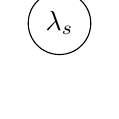
\begin{tikzpicture}[baseline=(char.base)]
\node(char)[draw,shape=circle]{$\lambda_s$};
\end{tikzpicture}\\
\cline{1-5}
\end{tabular}} \hspace{-0.3cm}\ar@{->}[r] &  \lambda_a} \\[0.6cm]
&\Rightarrow \,\, T \sim \text{Exponential}(\lambda_s-\lambda_a)\\[0.1cm]
{\footnotesize(\text{where $T$}} & {\footnotesize\text{ is the total time in the system)}}\\
\end{align*}

{\bf Normal Distribution:}\\[-0.6cm]
\begin{align*}
\bullet\quad X \sim \text{Normal}&(\mu,\sigma) \\[0.4cm]
\bullet\quad E(X) &= \mu \\[0.4cm]
\bullet\quad Var(X) &= \sigma^2 \\[0.4cm]
\bullet\quad (1-\alpha)100\% \text{ of the Normal}(\mu,\sigma) & \text{ distribution lies in } \mu \pm z_{\,\alpha/2}\,\,\sigma \\[0.4cm]
\bullet\quad \Pr(X > x) &= \Pr\left(Z> \frac{x-\mu}{\sigma}\right)\\[1cm]
\bullet\quad \Pr(Z < -z) &= \Pr(Z > z) \\[0.6cm]
\bullet\quad \Pr(Z > -z) &= \Pr(Z < z) = 1 -\Pr(Z>z) \\[1cm]
\bullet\quad \text{If} \,\,  X_1 \sim \text{Normal}(\mu_1,\sigma_1) \,\,  & \text{ and } \,\, X_2 \sim \text{Normal}(\mu_2,\sigma_2) \\[0.4cm]
\Rightarrow \quad  \text{ Sum: } \quad  X_1 + X_2 &\sim \text{Normal}\left(\mu_1+\mu_2,\,\sqrt{\sigma_1^2+\sigma_2^2}\,\right) \\[0.4cm]
\Rightarrow \quad  \text{ Difference: } \quad   X_1 - X_2 &\sim \text{Normal}\left(\mu_1-\mu_2,\,\sqrt{\sigma_1^2+\sigma_2^2}\,\right) \\[1cm]
\bullet\quad \text{For} \,\,  X_1,\ldots,X_n \sim \text{any distribution} & \text{ with } \mu = E(X) \text{ and } \sigma = Sd(X) = \sqrt{Var(X)}\\[0.4cm]
\Rightarrow \quad  \text{ Sample mean: } \quad  \,\overline{\!X} &\sim \text{Normal}\left(\mu,\,\frac{\sigma}{\sqrt{n}}\,\right) \quad \text{ if } n > 30
\end{align*}

\newpage


\section*{Useful Formulae: Page 4\\[0.3cm]}
{\bf Statistics and Standard Errors:}\\[0.1cm]
\begin{adjustwidth}{-2cm}{0cm}
\begin{tabular}{|c|c|c|c|c|}
\hline
&&&&\\[-0.1cm]
Parameter & Statistic & Standard Error & Samples & Details \\[0.3cm]
\hline
&&&&\\[-0.1cm]
$\mu$ & $\bar x$ & ${\displaystyle\frac{s}{\sqrt{n}}}$  & large / small & $\nu = n - 1$ \\[0.5cm]
\hline
&&&&\\[-0.1cm]
$p$ & $\hat p$ & \multirow{2}{*}{${\displaystyle\sqrt{\frac{\hat p\,(1-\hat p)}{n}}}$} & large & confidence \\[-0.1cm]
&&&&interval\\[0.3cm]
\cline{3-5}
&&&&\\[-0.1cm]
&  & \multirow{2}{*}{${\displaystyle\sqrt{\frac{p_0\,(1-p_0)}{n}}}$} & large & hypothesis \\[-0.1cm]
&&&&test\\[0.3cm]
\hline
&&&&\\[-0.1cm]
$\mu_1-\mu_2$ & $\bar x_1 - \bar x_2$ & \multirow{3}{*}{${\displaystyle\sqrt{\frac{s_1^2}{n_1}+\frac{s_2^2}{n_2}}}$} & large / small & ${\displaystyle \nu = \frac{(a+b)^2}{\frac{a^2}{n_1-1}+\frac{b^2}{n_2-1}}}$ \\[0.8cm]
&&&& ${\displaystyle a=\frac{s_1^2}{n_1}, \,\,\, b=\frac{s_2^2}{n_2}}$ \\[0.5cm]
\cline{3-5}
&&&&\\[-0.1cm]
&  & ${\displaystyle\sqrt{\frac{s_p^2}{n_1}+\frac{s_p^2}{n_2}}}$ & small & $\nu = n_1+n_2-2$ \\[0.5cm]
&&&& assuming \\[-0.2cm]
&& where\,\, ${\displaystyle s_p^2 = \frac{(n_1-1)\,s_1^2+(n_2-1)\,s_2^2}{n_1+n_2-2}}$  && $\sigma_1^2 = \sigma_2^2$ \\[0.5cm]
\hline
&&&&\\[-0.1cm]
$p_1-p_2$ & $\hat p_1 - \hat p_2$ & \multirow{2}{*}{${\displaystyle\sqrt{\frac{\hat p_1 \, (1-\hat p_1)}{n_1}+\frac{\hat p_2 \, (1-\hat p_2)}{n_2}}}$} & large & confidence\\[-0.1cm]
&&&&interval\\[0.5cm]
\cline{3-5}
&&&&\\[-0.1cm]
&  & ${\displaystyle\sqrt{\frac{\hat p_c\,(1-\hat p_c)}{n_1}+\frac{\hat p_c\,(1-\hat p_c)}{n_2}}}$ & large & hypothesis\\[-0.4cm]
&&&&test\\[0.2cm]
&&where\,\, ${\displaystyle \hat p_c = \frac{x_1+x_2}{n_1+n_2}}$&&\\[0.5cm]
\hline
\multicolumn{5}{c}{}\\[0.5cm]
\end{tabular}
\end{adjustwidth}
{\bf Confidence Intervals:}\\[-0.5cm]
\begin{align*}
\bullet\quad \text{Large sample:} \qquad \text{statistic } &\pm\,\, z_{\,\alpha/2}\,\times\,\text{standard error} \\[0.6cm]
\bullet\quad \text{Small sample:} \qquad \text{statistic } &\pm\,\, t_{\,\nu,\,\alpha/2}\,\times\,\text{standard error}
\end{align*}

\newpage

\section*{Useful Formulae: Page 5\\[0.3cm]}
{\bf Hypothesis Testing:}\\[-0.5cm]
\begin{align*}
\bullet\quad z &= \frac{\text{statistic}-\text{hypothesised value}}{\text{standard error}} \\[1cm]
\bullet\quad \text{p-value } &= \left\{
\begin{array}{rl}
2 \times \Pr(Z > |z|) & \text{if }  H_a: \, \mu \ne \mu_0\\[0.4cm]
\Pr(Z < z) & \text{if } H_a: \, \mu < \mu_0\\[0.4cm]
\Pr(Z > z) & \text{if } H_a: \, \mu > \mu_0\\
\end{array} \right.\\[1cm]
\bullet\quad F &= \frac{\text{larger variance}}{\text{smaller variance}} = \frac{s_{\text{larger}}^2}{s_{\text{smaller}}^2} \\[0.5cm]
 & \nu_1 = n_{\text{\,top}} - 1,\quad\, \nu_2 = n_{\text{\,bottom}} - 1 \\[1cm]
\bullet\quad \chi^2 &= \sum \frac{(o_i-e_i)^2}{e_i}\\[0.5cm]
\text{Goodness-of-fit: } \qquad &e_i = \text{total} \times p(x_i),\qquad \nu = n_f - 1- k \\[0.6cm]
\text{Independence: } \qquad &e_{ij} = \frac{r_i\,\times\,c_j}{\text{total}},\qquad \nu = (n_r - 1)\,\times\,(n_c - 1)\\[0.3cm]
\end{align*}
{\bf Information Theory:}\\[-0.5cm]
\begin{align*}
\bullet\quad h(x) &= - \log_2[p(x)] \\[0.6cm]
\bullet\quad H(X) &= E[h(X)] = \sum h(x_i)\,p(x_i) \\[1cm]
\bullet\quad l(x_i) &= \text{code-length for character } x_i \\[0.6cm]
\bullet\quad E(L) &= \sum l(x_i)\,p(x_i) \\[1cm]
\bullet\quad e &= \frac{H(X)}{E(L)} \\[1cm]
\bullet\quad &\sum 2^{-l(x_i)}  \le 1
\end{align*}


\end{document} 